\documentclass[11pt]{article}
\usepackage[utf8]{inputenc} 
\usepackage[T1]{fontenc}    
\usepackage{url}            
\usepackage{booktabs}       
\usepackage{amsfonts}       
\usepackage{nicefrac}       
\usepackage{microtype}      
\usepackage{fullpage}
\usepackage{subcaption}
\usepackage[most]{tcolorbox}
\usepackage[numbers]{natbib}
%\usepackage[textsize=tiny]{todonotes}
\setlength{\marginparwidth}{11ex}

\newcommand{\E}{\mathbb E}
\usepackage{wrapfig}
\usepackage{caption}

\newcommand{\theHalgorithm}{\arabic{algorithm}}

\usepackage{url}

\usepackage[utf8]{inputenc}
\usepackage{amsmath}
\usepackage{graphicx}
\usepackage{upgreek}
\usepackage{amsfonts}
\usepackage{amssymb}
\usepackage{amsthm}
\usepackage[mathscr]{euscript}
\usepackage{mathtools}
\newtheorem{thm}{Theorem}
\newtheorem{defn}{Definition}
\newtheorem{cor}{Corollary}
\newtheorem{assumption}{Assumption}
\newtheorem{lem}{Lemma}
\usepackage{xcolor}
\usepackage{nicefrac}
\usepackage{xr}
%\usepackage{chngcntr}
\usepackage{apptools}
\usepackage[page, header]{appendix}
\AtAppendix{\counterwithin{lem}{section}}
\usepackage{titletoc}
\usepackage{enumitem}
\setlist[itemize]{leftmargin=1cm}
\setlist[enumerate]{leftmargin=1cm}




\definecolor{DarkRed}{rgb}{0.75,0,0}
\definecolor{DarkGreen}{rgb}{0,0.5,0}
\definecolor{DarkPurple}{rgb}{0.5,0,0.5}
\definecolor{Dark}{rgb}{0.5,0.5,0}
\definecolor{DarkBlue}{rgb}{0,0,0.7}
\usepackage[bookmarks, colorlinks=true, plainpages = false, citecolor = DarkBlue, urlcolor = blue, filecolor = black, linkcolor =DarkGreen]{hyperref}
\usepackage{breakurl}
\usepackage[ruled, vlined, linesnumbered]{algorithm2e}
\newcommand\mycommfont[1]{\footnotesize\ttfamily\textcolor{blue}{#1}}
\SetCommentSty{mycommfont}

\DeclareMathOperator*{\argmin}{arg\,min}
\DeclareMathOperator*{\argmax}{arg\,max}

\allowdisplaybreaks[2]
\newcommand{\prob}{\mathbb P}
\newcommand{\Var}{\mathbb V}
\newcommand{\NN}{\mathbb N}
\newcommand{\Ex}{\mathbb E}
\newcommand{\varV}{\mathscr V}
\newcommand{\indicator}[1]{\mathbb I\{ #1 \} }
\newcommand{\statespace}{\mathcal S}
\newcommand{\actionspace}{\mathcal A}
\newcommand{\saspace}{\statespace \times \actionspace}
\newcommand{\satspace}{\mathcal Z}
\newcommand{\numsa}{\left|\saspace\right|}
\newcommand{\numsat}{\left|\satspace\right|}
\newcommand{\numS}{S}
\newcommand{\numA}{A}
\newcommand{\wmin}{w_{\min}}
\newcommand{\wminc}{w'_{\min}}
\newcommand{\range}{\operatorname{rng}}
\newcommand{\polylog}{\operatorname{polylog}}
\newcommand{\dspace}{\mathcal D}
\newcommand{\numD}{|\dspace|}
\newcommand{\numSucc}[1]{|\statespace(#1)|}
\newcommand{\succS}[1]{\statespace(#1)}

\newcommand{\reals}{\mathbb R}
\newcommand{\const}{\textrm{const.}}
\newcommand{\set}[1]{\left\{#1\right\}}
\newcommand{\llnp}{\operatorname{llnp}}
\newcommand{\defeq}{:=}
\usepackage{xspace}
\newcommand{\algname}{UBEV\xspace}

\mathtoolsset{showonlyrefs=true}

\let\temp\epsilon
\let\epsilon\varepsilon
\newcommand{\cK}{\mathcal K}
\newcommand{\cI}{\mathcal I}
\newcommand{\Pro}{\mathbb P}

\title{CS 234 Winter 2021 \\ Assignment 1 \\ Due: January 22 at 6:00 pm (PST)}
\date{}

\begin{document}
  \maketitle
\noindent For submission instructions please refer to \href{http://web.stanford.edu/class/cs234/assignments.html}{website}
For all problems, if you use an existing result from either the literature or a textbook to solve the exercise, you need to cite the source.



\section{Flappy Karel MDP [25 pts]}

There is a hot new mobile game on the market called Flappy Karel, where Karel the robot must dodge the red pillars of doom and flap its way to the green pasture. Consider the following 2 grid environments (Flappy World \ref{fig:fig1} and Flappy World \ref{fig:fig2}). Starting from any unshaded square, Karel can either move right $\&$ up, or  right $\&$ down (e.g from state 4 you can move to state 10 or 12, think checkers). Actions are deterministic and always succeed unless they will cause Karel to run into a wall. The thicker edges indicate walls, and attempting to move in the direction of a wall results in falling down one square (e.g. going in any direction from state 30 leads to falling into state 31). A successful run by Karel in Flappy World 1 is shown in Figure \ref{fig:fig1.b}. Taking any action from the green target squares (no. 32) earns a reward of $r_g$  and ends the episode. Taking any action from the red squares of doom (no. 1, 7, 8, 12, 13...) earns a reward of $r_r$ and ends the episode. Otherwise, from every other square, taking any action is associated with a reward $r_s$. Assume the discount factor $\gamma = 0.9$, $r_g = +5$, and $r_r = -5$ unless otherwise specified. Notice the Horizon is technically infinite in both worlds. 


\begin{figure}[ht]
\begin{subfigure}{.5\textwidth}
  \centering
  % include first image
  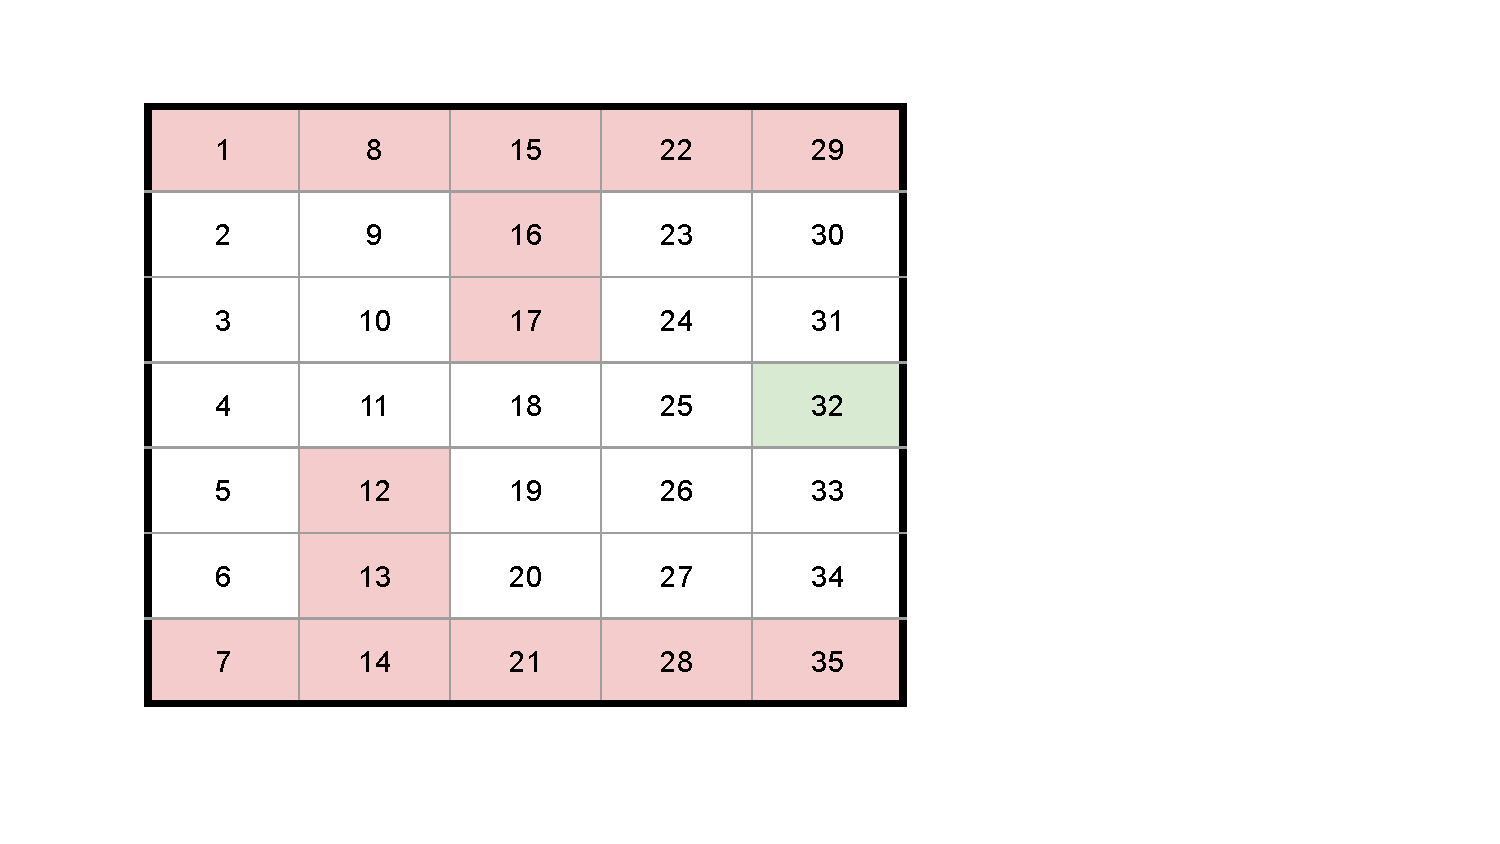
\includegraphics[width=.8\linewidth]{FlappyWorld1.pdf}  
  \caption{Flappy World 1}
  \label{fig:fig1.a}
\end{subfigure}
\begin{subfigure}{.5\textwidth}
  \centering
  % include second image
  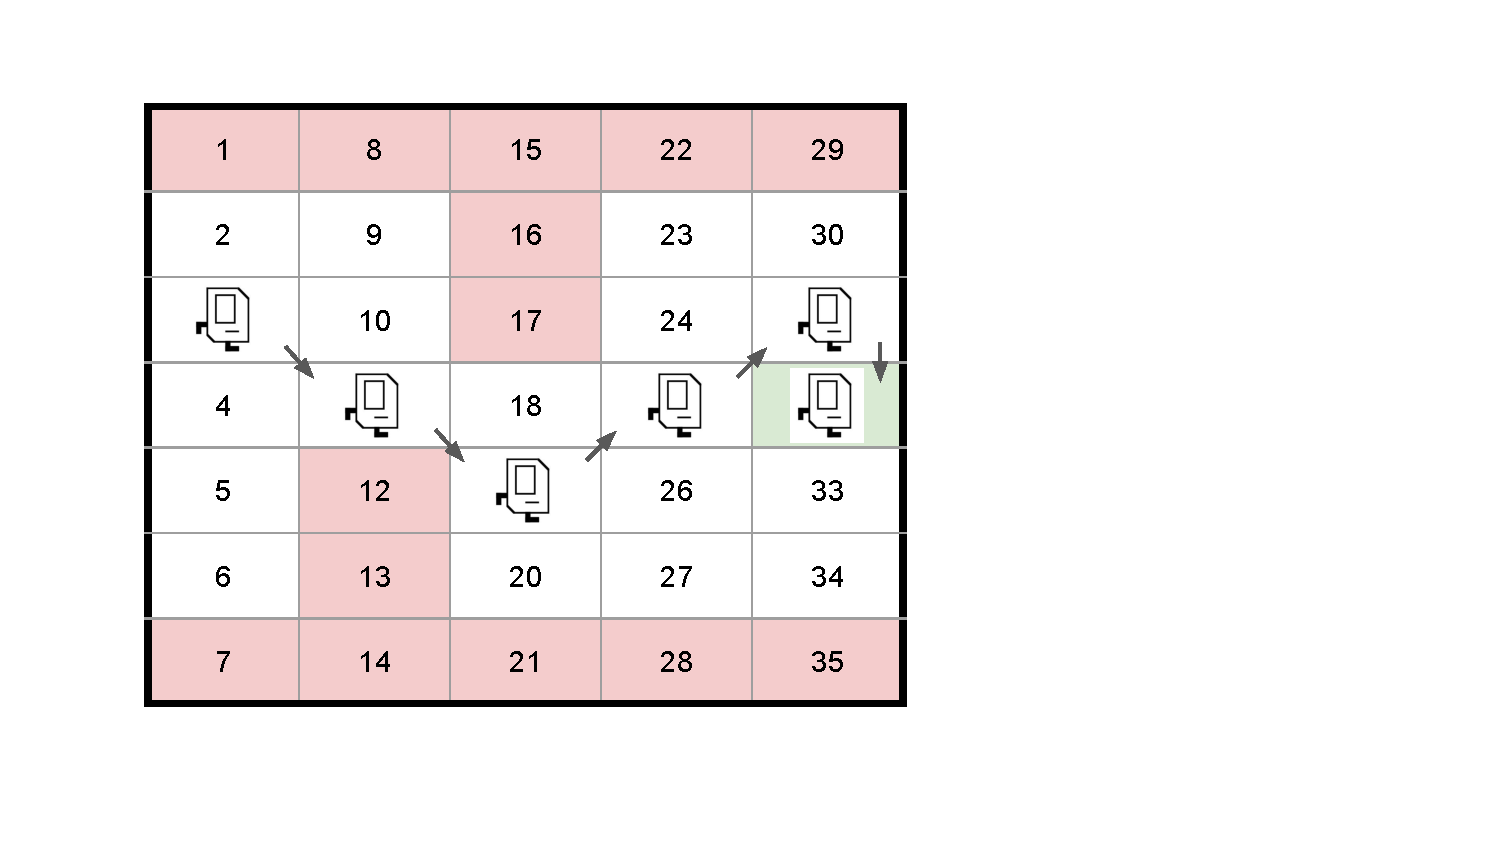
\includegraphics[width=.8\linewidth]{FlappyWorld1_.pdf}  
  \caption{A successful run by Karel in Flappy World 1}
  \label{fig:fig1.b}
\end{subfigure}
\caption{}
\label{fig:fig1}
\end{figure}

\begin{enumerate}[label=(\alph*)]
\item  Let $r_s \in \{-4,-1,0,1\}$. Starting in \textbf{square 2}, for each of the possible values of $r_s$ briefly explain what the optimal policy would be in Flappy World 1. In each case is the optimal policy unique and does the optimal policy depend on the value of the discount factor $\gamma$? Explain your answer.   [5 pts]


\item What value of $r_s$ would cause the optimal policy to return the shortest path to the green target square? Using this value of $r_s$ find the optimal value function for each square in Flappy world 1. What is the optimal action from square 27?  [5 pts]


\end{enumerate}

\noindent Now consider Flappy world 2. It is the same as Flappy world 1, except there are no walls on the right and left sides. Going past the right end of flappy world 2 simply loops you to left hand side. Take a look at Figure \ref{fig:fig1.b} for a successful run by Karel in Flappy World 2.  

\begin{figure}[ht]
\begin{subfigure}{.5\textwidth}
  \centering
  % include first image
  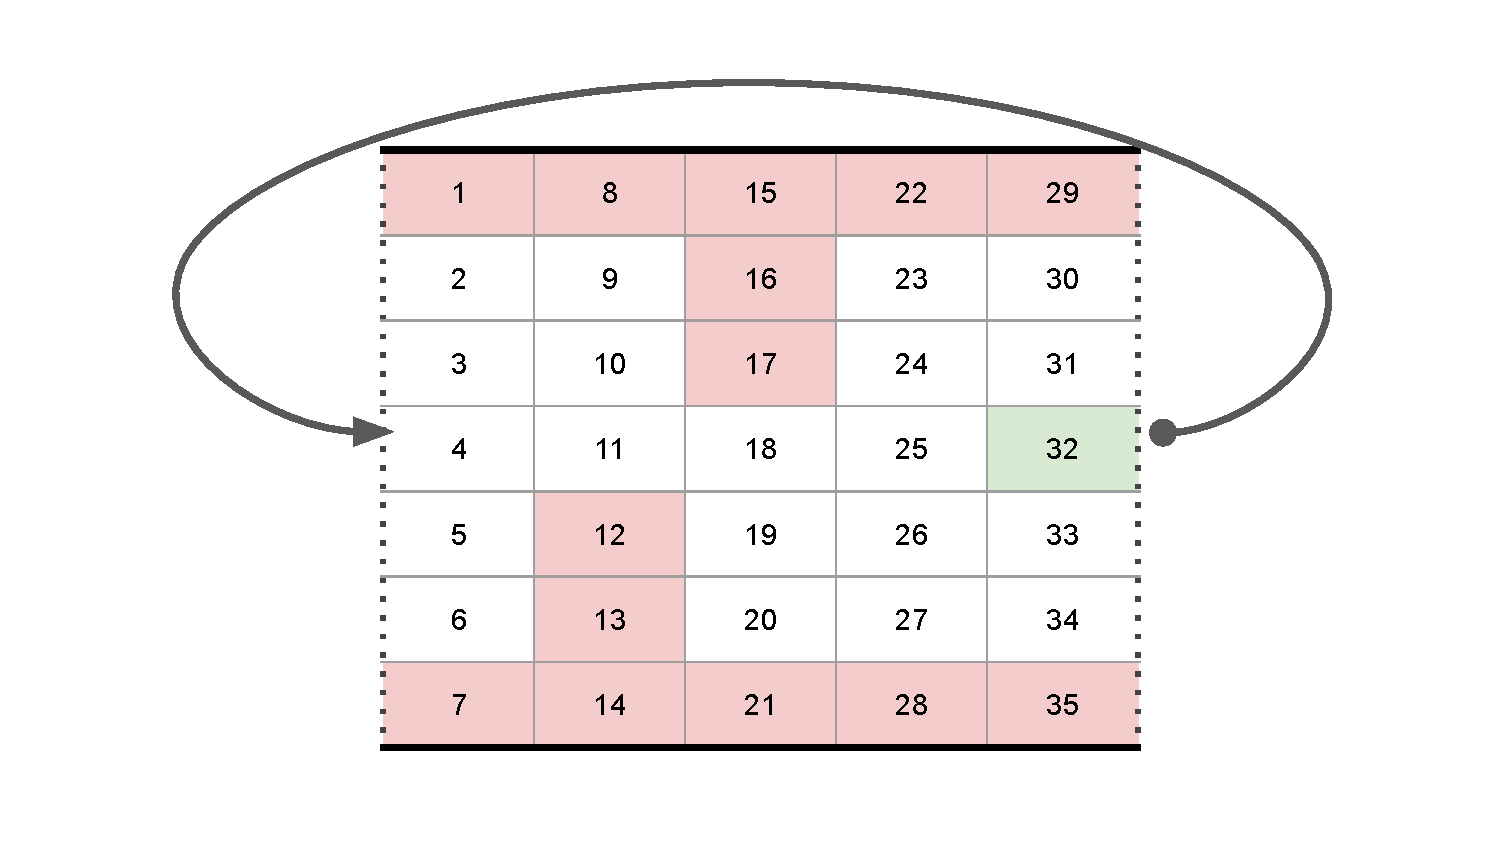
\includegraphics[width=.8\linewidth]{FlappyWorld2.pdf}  
  \caption{Flappy World 2}
  \label{fig:fig2.a}
\end{subfigure}
\begin{subfigure}{.5\textwidth}
  \centering
  % include second image
  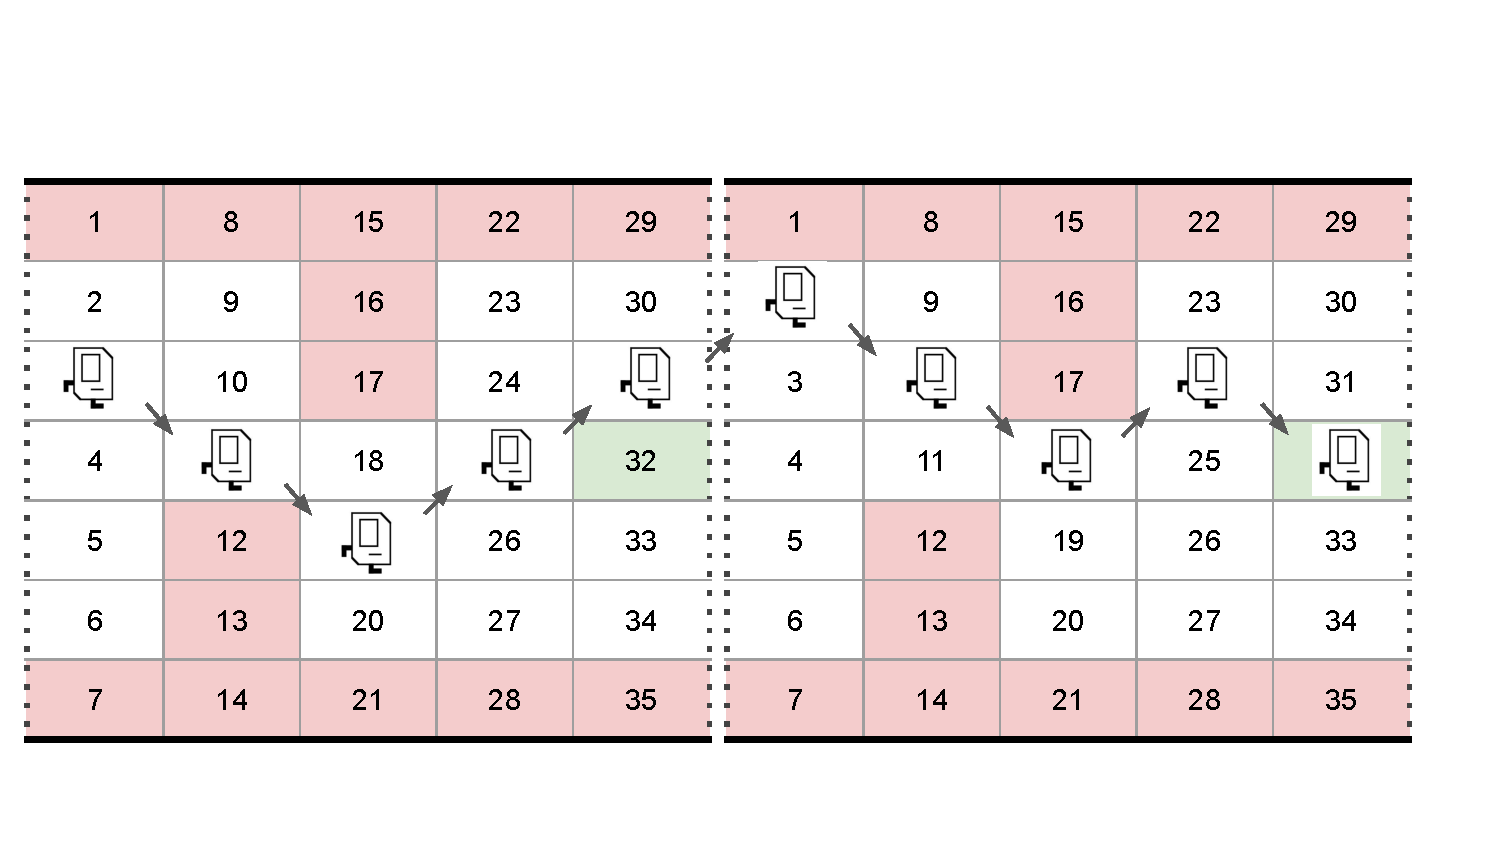
\includegraphics[width=.8\linewidth]{FlappyWorld2_.pdf}  
  \caption{A successful run by Karel in Flappy World 2}
  \label{fig:fig2.b}
\end{subfigure}
\caption{}
\label{fig:fig2}
\end{figure}

\begin{enumerate}

\item[(c)] Let $r_s \in \{-4,-1,0,1\}$. Starting in \textbf{square 3}, for each of the possible values of $r_s$ briefly explain what the optimal policy would be in Flappy World 2. Using the value of $r_s$, that would cause the optimal policy to return the shortest path to the green target square, find the optimal value function for each square in Flappy world 2. What is the optimal action from square 27? [5 pts]


\item[(d)] Consider a general MDP with rewards, and transitions. Consider a discount factor of $\gamma$. For this case assume that the horizon is infinite (so there is no termination). A policy $\pi$ in
this MDP induces a value function $V^{\pi}$ (lets refer to this as $V^{\pi}_{old}$ ). Now suppose we have the same MDP where all rewards have a constant $c$ added to them and then have been scaled by a constant $a$ (i.e. $r_{new} = a(c+ r_{old})$). Can you come up with an expression for the new value function $V^{\pi}$ induced by $\pi$ in this second MDP in terms of $V^{\pi}_{old}, c, a$, and $\gamma$? [5 pts]

\item[(e)] Can scaling all the rewards by a fixed amount change the optimal policy of a MDP? If so, describe how different ranges of the constant $a$ (where $r_{new} = a*(r_{old})$) would change the optimal policy of the MDP from part (c). [5 pts]

% \item[(f)] Now consider that instead of having a stationary target square the location can vary from time step to next time step. Let square no. 31 be the target with probability $\delata$ and square no. 31 be the target with probability $1 - \delata$ for some $delta in (0,1)$. Would a deterministic policy still be optimal in Flappy world 1? How about Flappy World 2? (assume $r_s=0$)  [5 pts]

\end{enumerate}


\begin{tcolorbox}[breakable]

\begin{enumerate}[label=(\alph*)]
    \item $r_s = 1$ Take longest possible path (2,10,18,24,30,31,32) to target square.\\
    $r_s = 0$ Take shortest possible path to target square. \\
    $r_s = -1$ Take shortest possible path to target square. \\
    $r_s = -4$ Take shortest possible path to a red square. \\ \\
    In general the optimal policy is not unique and depends on $\gamma$ (think what would happen if $\gamma = 0$) . In this case for $r_s = -1$ multiple equivalent optimal policies exist (not counting actions in the terminal states).\\
    
    
    \item $r_s = -1$\\
    \begin{tabular}{ | c | c | c | c | c | }
    \hline
    -5     &  -5   &   -5    &   -5   &    -5 \\
    \hline
    -0.1585 & -5.5  &   -5    &   2.15 &    2.15   \\
    \hline
    -1.14265 &  0.935 &   -5    &   3.5  &    3.5    \\
    \hline
    -0.1585 & -0.1585 &   2.15  &   2.15 &    5     \\
    \hline
    -1.14265 & -5    &   0.935 &   3.5  &   -5.95   \\
    \hline
    -5.5    & -5    &  2.15   &  -5.5  &   -5.5    \\
    \hline
    -5     & -5    &  -5    &  -5   &   -5     \\
    \hline
    \end{tabular}
    \\ 
    Right \& Down is the optimal action from square 27\\
    \\
    \\
    \\
    $r_s = 0$\\ 
    \begin{tabular}{ | c | c | c | c | c | }
    \hline
    -5     &  -5   &   -5    &   -5   &    -5 \\
    \hline
    3.2805 & -4.5   &  -5.   &    4.05  &   4.05 \\
    \hline
    2.95245 & 3.645 &  -5.    &   4.5   &   4.5   \\
    \hline
    3.2805  & 3.2805 &  4.05  &   4.05  &   5.     \\
    \hline
    2.95245 &-5.    &   3.645  &  4.5   &  -4.05   \\
    \hline
    -4.5    & -5.   &    4.05  &  -3.645 &  -4.5   \\
    \hline
    -5     & -5    &  -5    &  -5   &   -5     \\
    \hline
    \end{tabular}\\ 
    Right \& up is the optimal action from square 27\\
    
    \item
    $r_s = 1$ Loop infinitely.\\
    $r_s = 0$ Take shortest possible path to target square. \\
    $r_s = -1$ Take shortest possible path to target square. \\
    $r_s = -4$ Take shortest possible path to a red square. \\ 
    \\
    \\
    \\
    $r_s = -1$\\ 
    \begin{tabular}{ | c | c | c | c | c | }
    \hline
    -5.       &  -5.     &    -5.    &     -5.      &   -5.        \\
    \hline
    -0.1585   &  -5.5    &    -5.    &     -2.028385 &  -4.7698234 \\
    \hline
    -4.18869267 & 0.935  &   -5.     &     3.5     &   -1.14265   \\
    \hline
    -0.1585   &  -3.54299185 & 2.15   &    -2.028385 &   5.        \\
    \hline
    -4.18869267 & -5.    &     -2.8255465 &  3.5   &     -1.14265   \\
    \hline
    -5.5      &  -5.     &     2.15    &   -2.028385 &  -4.7698234 \\
    \hline
    -5.       &  -5.      &   -5.    &    -5.    &     -5.      \\
    \hline
    \end{tabular}
    \\
    Right \& Up is the optimal action from square 27\\
        \\
    \\
    \\
    $r_s = 0$\\ 
    \begin{tabular}{ | c | c | c | c | c | }
    \hline
    -5.       &  -5.     &    -5.    &     -5.      &   -5.        \\
    \hline
    3.2805   &  -4.5     &   -5.     &     2.657205 &   1.7433922 \\
    \hline
    1.93710245 & 3.645   &   -5.     &     4.5      &   2.95245   \\
    \hline
    3.2805    &  2.15233605 & 4.05    &    2.657205  &  5.      \\
    \hline
    1.93710245 &-5.      &    2.3914845  & 4.5      &   2.95245  \\
    \hline
    -4.5      &  -5.     &     4.05    &    2.657205 &   1.7433922\\
    \hline
    -5.       &  -5.      &   -5.    &    -5.    &     -5.      \\
    \hline
    \end{tabular}
    \\
    Right \& Up is the optimal action from square 27\\
    
    
    \item $V^{\pi}_{new} = a* V^{\pi}_{old} + \frac{a*c}{1-\gamma}$
    
    \item Yes, it can change the optimal policy. Choosing a<0 would reverse the order, making the previously worse policy optimal. Setting a = 0 would make all policies optimal. 
\end{enumerate}

\end{tcolorbox}

\newpage

\section{Applications of the Performance Difference Lemma [20pts]}

%In many situations such as healthcare or education, we cannot run any arbitrary policy and collect data from running those policies for evaluation. In these cases, we may need to take data collected from following one policy and use it to evaluate the value of a different policy. The equality proved in the following exercise can be an important tool for achieving this.
The purpose of this exercise is to get familiar on how to compare the value of different policies, $\pi_1$ and $\pi_2$, on a fixed horizon MDP. A fixed horizon MDP is an MDP where the agent's state is reset after $H$ timesteps; $H$ is called the \emph{horizon} of the MDP. There is no discount (i.e., $\gamma=1$) and policies are allowed to be non-stationary, i.e., the action identified by a policy depends on the timestep in addition to the state.
Let $x_t\sim \pi$ denote the distribution over states at timestep $t$ (for $1\leq t \leq H$) upon following policy $\pi$ and $V^{\pi}_t(x_t)$ denote the value function of policy $\pi$ in state 
$x_t$ and timestep $t$, and $Q_t^{\pi}(x_t,a)$ denote the corresponding 
$Q$ value associated to action $a$. As a clarifying example, we denote $\E_{x_t \sim \pi_1} V(x_t)$ to represent the average value of the value function $V(\cdot)$ over the states at timestep $t$ encountered upon following policy $\pi_1$. The following equality is called \emph{performance difference lemma} :
\begin{equation}
\label{eq:1}
V_1^{\pi_1}(x_1) - V_1^{\pi_2}(x_1) =  \sum_{t=1}^H \E_{x_t \sim \pi_2} \Big( Q_t^{\pi_1}(x_t,\pi_1(x_t,t)) - Q_t^{\pi_1}(x_t,\pi_2(x_t,t)) \Big)
\end{equation}

\textbf{Intuition:} The above expression can be interpreted in the following way. For concreteness, assume that $\pi_1$ is the better policy, i.e., achieving $V_1^{\pi_1}(x_1) \geq V_1^{\pi_2}(x_1)$. Suppose you're following policy $\pi_2$ and you are at timestep $t$ in state $x_t$. 
You have the option to follow $\pi_1$ (the better policy) until the end of the episode, totalling $Q_t^{\pi_1}(x_t,\pi_1(x_t,t))$ return from the current state-timestep; or you have the option to follow $\pi_2$ for one timestep and then follow $\pi_1$ instead until the end of the episode (you can follow many other policies of course). This would give you a ``loss'' of $Q_t^{\pi_1}(x_t,\pi_1(x_t,t)) - Q_t^{\pi_1}(x_t,\pi_2(x_t,t))$ that originates from following the worse policy $\pi_2$ instead of $\pi_1$ in that timestep. 
% Then equation \ref{eq:1} 
Then the equation above
means that the value difference of the two policies is the sum of all the losses induced by following the suboptimal policy for every timestep, weighted by the expected trajectory of the policy you're following.

\textbf{Question}
You will use the performance difference lemma to solve this problem. Consider an MDP where the state space $\mathcal S$ is partitioned into two sets of states $\mathcal S^+$ and its complement $\overline{\mathcal S}^+$.
\begin{align}
\mathcal S & = \mathcal S^+ \cup \overline{\mathcal S}^+ \\
\mathcal S^+ \cap \overline{\mathcal S}^+ & = \emptyset.
\end{align}

In every state $s \in \mathcal S^+$ there exists an action $a^+$ that leads to the same state with probability 1 and gives a unitary reward:
\begin{align}
    p(s_{t+1} = s \mid s_{t} =s,a_t=a^+) = 1, \quad \quad \quad p(s{t+1} \neq s \mid s_{t} =s,a_t=a^+) = 0.
\end{align}

The reward function is always positive. In $\mathcal S^+$ the reward function equals $1$ upon playing $a^+$ and $H$ upon playing any action $a \neq a^+$.  Therefore in $ \mathcal S^+$
\begin{align}
    r(s,a^+) = 1, \quad   r(s,a) = H, \quad  a \neq a^+
\end{align}
Conversely, in any state $s \not \in S^+$, the reward function is in $[0,1]$ ($\forall s \not \in S^+ \ \ \ \forall a \ \ r(s,a) \in [0,1]$).

Consider a deterministic policy $\pi$ and define a policy $\pi^+$ that takes action $a^+$ in any state $\mathcal S^+$ and is otherwise equal to $\pi$:
\begin{align}
    \pi^+(s) = a^+ \; \text{if} \; s \in \mathcal S^+, \quad \quad \pi^+(s) = \pi(s) \; \text{if} \; s \not\in \mathcal S^+
\end{align}
Intuitively, $\pi$ accumulates higher return than $\pi^+$: in any state in $\mathcal S^+$ the policy $\pi^+$ chooses to take a unitary reward forever instead of a reward of $H$ and then maybe more.
Using the performance difference lemma show that at any state $s_0$
\begin{align}
    V^{\pi}_{1}(s_0) \geq  V^{\pi^+}_{1}(s_0).
\end{align}


\begin{tcolorbox}[breakable]

For any $t =1,2,\dots H$ we can write
\begin{align}
  (V_t^{\pi^+} - V_t^{\pi})(s_0) & = \E_{(s,a) \sim \pi} \Big[(Q_t^{\pi^+}(s,\pi^+(s)) - Q_t^{\pi^+}(s,a))\mathbb{I}\{s \in \mathcal S^+ \cap a \neq a+ \}\Big]\\
  &  + \E_{(s,a) \sim \pi} \Big[(Q_t^{\pi^+}(s,\pi^+(s)) - Q_t^{\pi^+}(s,a))\mathbb{I}\{s \not \in \mathcal S^+ \cap a \neq a+\} \Big]\\
  & = \E_{(s,a) \sim \pi} \Big[(Q_t^{\pi^+}(s,\pi^+(s)) - Q_t^{\pi^+}(s,a))\mathbb{I}\{s \in \mathcal S^+\cap a \neq a+ \}\Big]\\ 
  & \leq \E_{(s,a) \sim \pi} \Big[(H - H -  \E_{s' \sim p(s,a)}V_{t+1}^{\pi^+}(s'))\mathbb{I}\{s \in \mathcal S^+\cap a \neq a+ \}\Big] \leq 0,\\
\end{align}

\end{tcolorbox}

\newpage


\section{Nonstationary Discount Factor $\gamma$ [30 pts]}

In this problem you will consider a variable discount factor $\gamma$. In lecture 2, we proved that the Bellman backup is a contraction for $\gamma < 1$ in the infinity norm. 

In this problem we consider having a non-stationary discount factor and assume you want to run $K$ iterations of value iterations. Let $V_K$ and $V'_K$ be any two arbitrary initial value functions (at timestep $K$).
The time-dependent Bellman backup operator $B_k$ is defined as
\begin{equation}
    V_{k-1} \overset{def}{=} B_{k}V_{k} = \max_a[ R(s, a) + \gamma_k\sum_{s' \in S}p(s'|s,a)V_{k}(s')]
\end{equation}
where
\begin{equation}
    \gamma_{k} = 1 - \frac{1}{k+1}
\end{equation}
Notice that the value function index is decreasing: $K,K-1,\dots,2,1$

\begin{enumerate}
\item [10pt] Similarly to what you've done in class, show that the Bellman operator with non-stationary discount factor at time step k is still a contraction, i.e.,  
\begin{align}
\| B_k V - B_k V' \|_\infty
\leq \gamma_k \|V - V' \|_\infty
\end{align}
\item [10pt] Using the above inequality prove that
\begin{align}
\| B_1B_2 \cdots B_K V_K -  B_1B_2 \cdots B_K V'_K \|_\infty
\leq \gamma_1 \gamma_2 \cdots \gamma_k \|V_K - V'_K \|_\infty
\end{align}
\item [10pt] Unfortunately $\gamma_k \approx 1$ when $k$ is large so you cannot conclude that the convergence occurs exponentially fast. However, the error still shrinks: show that
\begin{align}
  \gamma_1 \gamma_2 \cdots \gamma_K = \frac{1}{K+1}
\end{align}
which allows you to write
\begin{align}
\| B_1B_2 \cdots B_K V_K -  B_1B_2 \cdots B_K V'_K \|_\infty \leq \frac{1}{K+1} \|V_K - V'_K \|_\infty
\end{align}
and ensure convergence, albeit at a slower rate.
\end{enumerate}


\begin{tcolorbox}[breakable]


\begin{enumerate}
\item 
\begin{align}
\| B_k V - B_k V' \|_\infty 
& = \| \max_a[ R(s, a) + \gamma_k\sum_{s' \in S}p(s'|s,a)V_{k}(s')] \\ & - \max_a[ R(s, a) + \gamma_k\sum_{s' \in S}p(s'|s,a)V_{k}'(s')] \|_\infty \\
& \leq \max_a\| \gamma_k\sum_{s' \in S}p(s'|s,a)(V_{k}(s') - V_{k}'(s')) \|_\infty \\
& \leq \max_a\| \gamma_k\|V_{k} - V_{k}'\| \sum_{s' \in S}p(s'|s,a) \|_\infty \\
& = \gamma_k \|V - V' \|_\infty
\end{align}

\item 
\begin{align}
\| B_1(B_2 \cdots B_K V_K) -  B_1(B_2 \dots B_K V'_K) \|_\infty
& \leq \gamma_1 \| B_2 (B_3 \cdots B_K V_K) -   B_2 (B_3 \cdots B_K V'_K) \|_\infty \\
& \leq \gamma_1 \gamma_2 \| B_3 (B_4 \cdots B_K V_K) - B_3 (B_4 \cdots B_K V'_K) \|_\infty\\
& \cdots\\
& \leq \gamma_1 \gamma_2 \cdots \gamma_k \|V_K - V'_K \|_\infty\\
\end{align}

\item 
\begin{align}
\gamma_1 \gamma_2 \cdots \gamma_K 
& = (1 - \frac{1}{2})(1 - \frac{1}{3})(1 - \frac{1}{4}) \cdots (1 - \frac{1}{k+1})\\
& = (\frac{1}{2})(\frac{2}{3})(\frac{3}{4}) \cdots (\frac{k}{k+1}) \\
&= \frac{1}{K+1}
\end{align}
\end{enumerate}


\end{tcolorbox}


\newpage

\begin{section}{Frozen Lake MDP [25 pts]}
Now you will implement value iteration and policy iteration for the Frozen Lake environment
from \href{"https://gym.openai.com/envs/FrozenLake-v0"}{OpenAI Gym}. We have provided
custom versions of this environment in the starter code.
\begin{enumerate}[label=(\alph*)]
\item \textbf{(coding)} Read through \texttt{vi\_and\_pi.py} and implement \texttt{policy\_evaluation}, \texttt{policy\_improvement} and \texttt{policy\_iteration}. The stopping tolerance (defined as $\max_s |V_{old}(s) - V_{new}(s)|$) is tol = $10^{-3}$
. Use $\gamma = 0.9$. Return the optimal value function and the optimal policy. [10pts]
\item \textbf{(coding)} Implement \texttt{value\_iteration} in \texttt{vi\_and\_pi.py}. The stopping tolerance is tol =
$10^{-3}$
. Use $\gamma = 0.9$. Return the optimal value function and the optimal policy. [10 pts]
\item \textbf{(written)} Run both methods on the Deterministic-4x4-FrozenLake-v0 and

Stochastic-4x4-FrozenLake-v0 environments. In the second environment, the dynamics of the world are stochastic. How does stochasticity affect the number of iterations required, and the resulting policy? [5 pts]

\end{enumerate}
\end{section}

\begin{tcolorbox}[breakable]
\begin{enumerate}
    \item[(c)] Stochasticity generally increases the number of iterations required to converge. In the stochastic frozen lake environment, the number of iterations for value iteration increases. For policy iteration, depending on the implementation method, the number of iterations could remain unchanged; or policy iteration might not even converge at all. The stochasticity would also change the optimal policy. In this environment, the optimal policy of the stochastic frozen lake is different from the one of the deterministic frozen lake.
\end{enumerate}


\end{tcolorbox}



\end{document} 